\documentclass[10pt,a4paper]{article}
\usepackage[margin=0.62in]{geometry}
\usepackage[T1]{fontenc}
\usepackage[utf8]{inputenc}
\usepackage{lmodern}
\usepackage{amsmath,amssymb}
\usepackage{booktabs}
\usepackage{tabularx}
\usepackage{array}
\usepackage{graphicx}
\usepackage{float}
\usepackage{subcaption}
\usepackage{enumitem}
\usepackage{xcolor}
\usepackage{hyperref}
\usepackage{microtype}
\usepackage{titlesec}
\usepackage{fancyhdr}
\usepackage[most]{tcolorbox}
\usepackage{tikz}
\usetikzlibrary{positioning,arrows.meta,calc,shapes.geometric,decorations.pathreplacing,fit}

\definecolor{brand}{HTML}{0D3B66}
\definecolor{accent}{HTML}{2A9D8F}
\definecolor{softbg}{HTML}{F4F8FB}
\definecolor{textdark}{HTML}{1E1E1E}

\hypersetup{
  colorlinks=true,
  linkcolor=brand,
  urlcolor=accent
}

\setlength{\parindent}{0pt}
\setlength{\parskip}{3pt}
\setlist[itemize]{leftmargin=1.2em,itemsep=1pt,topsep=2pt}

\titleformat{\section}{\color{brand}\large\bfseries}{\thesection.}{0.4em}{}
\titleformat{\subsection}{\color{textdark}\bfseries}{\thesubsection}{0.4em}{}
\titlespacing*{\section}{0pt}{8pt}{4pt}
\titlespacing*{\subsection}{0pt}{6pt}{3pt}

\pagestyle{fancy}
\fancyhf{}
\fancyhead[L]{\small CS671 Technical Model Report}
\fancyhead[R]{\small Unpaired Diffusion (Brain)}
\fancyfoot[C]{\small \thepage}
\setlength{\headheight}{14pt}

\begin{document}

% -------------------- Header Block --------------------
\begin{tcolorbox}[
  enhanced,
  colback=softbg,
  colframe=brand,
  boxrule=0.9pt,
  arc=2mm,
  left=5pt,right=5pt,top=5pt,bottom=5pt
]
\centering
{\Large\bfseries\color{brand} CS671 -- Deep Learning and Its Applications}\\[2pt]
{\large\bfseries Technical Documentation Report}\\[6pt]
{\normalsize\bfseries Model: Unpaired Diffusion (Brain)}\\[4pt]
\small
Project Group: 5 \quad Region: Brain \quad Modality: Unpaired (CT $\leftrightarrow$ MRI)
\end{tcolorbox}

\section{ARCHITECTURAL OVERVIEW}
Unpaired Diffusion (Cycle Diffusion) addresses the challenge of modality translation when spatially aligned pairs are unavailable. It combines the generative power of Latent Diffusion Models (LDM) with the structural constraints of Cycle-Consistency. The model learns to map CT latents to MRI latents by ensuring that the transformation is reversible.

\subsection{Cycle-Consistent Latent Diffusion}
The architecture is implemented as a dual-path Latent Diffusion Model (LDM). It utilizes two distinct Variational Autoencoder (VAE) pathways, labeled \texttt{a2b} (CT to MRI) and \texttt{b2a} (MRI to CT), linked by a shared latent denoising UNet adapted via LoRA.

\begin{figure}[H]
\centering
\resizebox{\textwidth}{!}{
\begin{tikzpicture}[
    node distance=5mm and 12mm,
    block/.style={draw=brand, thick, fill=softbg, minimum width=2.4cm, minimum height=0.9cm, align=center, rounded corners=1mm, font=\scriptsize},
    module/.style={draw=accent, thick, fill=white, minimum width=2.2cm, minimum height=0.7cm, align=center, font=\tiny},
    arr/.style={-{Latex[length=1.5mm]}, thick, draw=brand!70},
    skip/.style={-{Latex[length=1.5mm]}, thick, dashed, draw=accent}
]
    % Domain A (CT) path
    \node[block] (ct) {Real CT};
    \node[module, right=of ct] (enc_a) {VAE Enc (a2b)\\+ Skip Features};
    \node[block, right=of enc_a, fill=accent!10] (za) {Latent $z_a$};
    
    % Shared Denoiser
    \node[draw=brand, thick, dashed, rounded corners=2mm, inner sep=5mm, right=2.8cm of za] (unet) {UNet2DConditionModel\\(LoRA Adapted)};
    
    % Domain B (MRI) path
    \node[block, right=2.8cm of unet, fill=accent!10] (zb) {Latent $z_b$};
    \node[module, right=of zb] (dec_b) {VAE Dec (a2b)\\+ Skip Injection};
    \node[block, right=of dec_b] (mri) {Fake MRI};

    % Connections
    \draw[arr] (ct) -- (enc_a); \draw[arr] (enc_a) -- (za);
    \draw[arr] (za) -- (unet) node[midway, above, font=\tiny] {CT Latent Cond.};
    \draw[arr] (unet) -- (zb) node[midway, above, font=\tiny] {Denoise};
    \draw[arr] (zb) -- (dec_b); \draw[arr] (dec_b) -- (mri);

    % Cycle path
    \draw[arr, dashed, rounded corners=3mm] (zb.south) -- ++(0,-1.2) -| (za.south) node[pos=0.25, below, font=\tiny] {Reverse Translation ($b \to a$) for Cycle Consistency};
\end{tikzpicture}
}
\caption{Dual-Path Latent Diffusion: Modality translation is achieved by conditioning the denoising process on the encoded latent of the source domain, with cycle-consistency enforced to ensure anatomical invariance.}
\end{figure}

\textbf{Anatomical Preservation via Latent Cycle-Consistency:} 
The implementation enforces structural fidelity by requiring that a CT latent encoded through the \texttt{a2b} path and translated back via the \texttt{b2a} path remains close to the original latent. This latent-space cycle-consistency is significantly more stable than pixel-space cycles, as it allows the model to focus on high-level anatomical features rather than noise-level variance.

\textbf{VAE Skip-Injection and LoRA Adapters:} 
Similar to the paired model, the unpaired implementation overrides the VAE's \texttt{encoder.forward} and \texttt{decoder.forward} to include custom skip connections. These connections project intermediate feature maps using learned $1 \times 1$ convolutions to provide the decoder with "anatomical shortcuts." Both the UNet and VAE paths are fine-tuned using Low-Rank Adaptation (LoRA), which allows the model to learn the specific CT-to-MRI mapping of the SynthRAD dataset while preserving the pre-trained generative priors of the base diffusion model.

\section{TRAINING DYNAMICS}
The training objective combines latent-level adversarial losses with cycle-consistency constraints.

\begin{figure}[H]
\centering
\resizebox{0.8\textwidth}{!}{
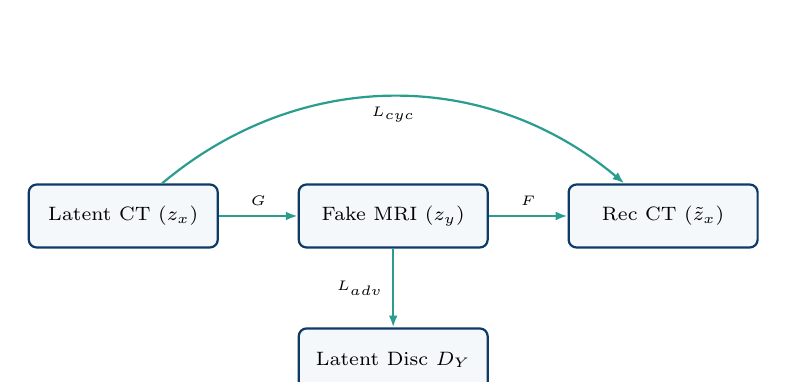
\begin{tikzpicture}[
    node distance=10mm,
    box/.style={draw=brand, thick, fill=softbg, minimum width=2.4cm, minimum height=0.8cm, align=center, rounded corners=1mm, font=\scriptsize},
    arr/.style={-{Latex[length=1.5mm]}, thick, draw=accent}
]
    \node[box] (zx) {Latent CT ($z_x$)};
    \node[box, right=of zx] (zy) {Fake MRI ($z_y$)};
    \node[box, right=of zy] (recx) {Rec CT ($\tilde{z}_x$)};
    
    \draw[arr] (zx) -- (zy) node[midway, above, font=\tiny] {$G$};
    \draw[arr] (zy) -- (recx) node[midway, above, font=\tiny] {$F$};
    \draw[arr, bend left=40] (zx) to node[midway, below, font=\tiny] {$L_{cyc}$} (recx);

    \node[box, below=1cm of zy] (disc) {Latent Disc $D_Y$};
    \draw[arr] (zy) -- (disc) node[midway, left, font=\tiny] {$L_{adv}$};
\end{tikzpicture}
}
\caption{Unpaired Diffusion Training: Adversarial and Cycle-Consistency loops in latent space.}
\end{figure}

\textbf{Optimization and Latent Adversarial Loss:} 
The implementation minimizes a composite loss function including the standard LDM epsilon-prediction loss and a latent-space reconstruction loss. By utilizing a \texttt{DDPMScheduler} with a reduced timestep trajectory, the model achieves efficient unpaired translation. The LoRA rank and alpha parameters are specifically tuned to balance the trade-off between modality translation fidelity and the preservation of global brain anatomy.

\section{INFERENCE PIPELINE}
Inference involves encoding the CT volume, performing latent translation, and decoding the result.

\begin{figure}[H]
\centering
\resizebox{0.85\textwidth}{!}{
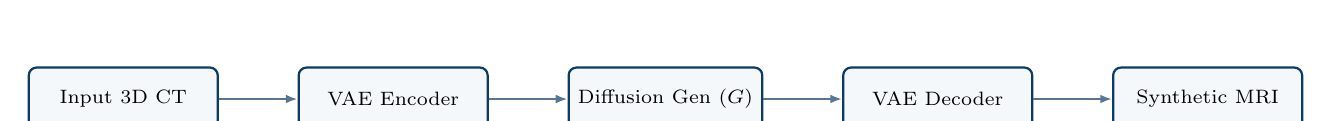
\begin{tikzpicture}[
    node distance=10mm,
    block/.style={draw=brand, thick, fill=softbg, minimum width=2.4cm, minimum height=0.8cm, align=center, rounded corners=1mm, font=\scriptsize},
    arr/.style={-{Latex[length=1.5mm]}, thick, draw=brand!70}
]
    \node[block] (in) {Input 3D CT};
    \node[block, right=of in] (e) {VAE Encoder};
    \node[block, right=of e] (g) {Diffusion Gen ($G$)};
    \node[block, right=of g] (d) {VAE Decoder};
    \node[block, right=of d] (out) {Synthetic MRI};

    \draw[arr] (in) -- (e);
    \draw[arr] (e) -- (g);
    \draw[arr] (g) -- (d);
    \draw[arr] (d) -- (out);
\end{tikzpicture}
}
\caption{Inference flow: End-to-end latent translation and reconstruction.}
\end{figure}

The inference engine processes the volume slice-by-slice. The CT latent is passed through the diffusion generator, which performs a set of denoising steps (guided by the CT latent itself) to produce a corresponding MRI latent. This latent is then decoded into the final image space.

\end{document}
